\chapter{Latex Einfuehrung}

Kurzeinführung zu Latex: \url{https://latex.tugraz.at/start}

Buch zu Latex: \url{https://en.wikibooks.org/wiki/LaTeX}

\section{Grafiken}


Grafiken werden mit dem Figure tag eingebunden. Sie können zentriert über die ganze Seite oder neben dem Text platziert werden.

\begin{figure}[h]
\begin{center}
\includegraphics[width=7cm]{Hexapod.png}
\caption{Hexapod}
\label{fig:hexapod}
\end{center}
\end{figure}

Grafik neben Text:

\begin{wrapfigure}{R}{0.5\linewidth}
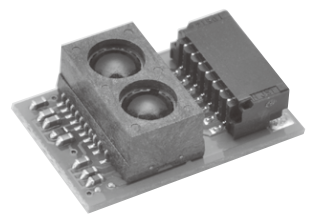
\includegraphics[scale=0.8]{GPE.png}
\caption{GP2Y0E03 \cite{GP2Y0E03}}
\label{fig:GPE}
\end{wrapfigure}

Lorem ipsum dolor sit amet, consectetur adipiscing elit, sed do eiusmod tempor incididunt ut labore et dolore magna aliqua. Ut enim ad minim veniam, quis nostrud exercitation ullamco laboris nisi ut aliquip ex ea commodo consequat. Duis aute irure dolor in reprehenderit in voluptate velit esse cillum dolore eu fugiat nulla pariatur. Excepteur sint occaecat cupidatat non proident, sunt in culpa qui officia deserunt mollit anim id est laborum. 
Lorem ipsum dolor sit amet, consectetur adipiscing elit, sed do eiusmod tempor incididunt ut labore et dolore magna aliqua. Ut enim ad minim veniam, quis nostrud exercitation ullamco laboris nisi ut aliquip ex ea commodo consequat. Duis aute irure dolor in reprehenderit in voluptate velit esse cillum dolore eu fugiat nulla pariatur. Excepteur sint occaecat cupidatat non proident, sunt in culpa qui officia deserunt mollit anim id est laborum. 


\section{Code Listings}
Code listings können mit verschiedenen packages erzeugt werden.

Code Listing:
\begin{lstlisting}[language=C++,caption=Example Code	]
  #include <stdio.h>
  
  int main (void) {
    printf("count: ");
    for (int i = 1; i <= 10; i++) {
     printf("%d ", i);
    }
    return 0;
  }
\end{lstlisting}


\bigskip
Alternatives Code Listing, floating, mit caption

\begin{listing}[H]
 \begin{minted}{c}
  #include <stdio.h>
  
  int main (void) {
    printf("count: ");
    for (int i = 1; i <= 10; i++) {
     printf("%d ", i);
    }
    return 0;
  }
  \end{minted}
  \caption{Example Code Caption}
\end{listing}

\bigskip 

Nicht Floating, ohne Caption:
\begin{minted}[label=``Example Code'']{c}
  #include <stdio.h>
  
  int main (void) {
    printf("count: ");
    for (int i = 1; i <= 10; i++) {
     printf("%d ", i);
    }
    return 0;
  }
\end{minted}



\section{Zitieren in Latex}
Latex nutzt Bibtex für die Verwaltung von Literaturquellen. In der Vorlage existiert bereits die Datei Literatur.bib mit zwei Einträgen. Ein Eintrag aus der Bibtex Datei kann mit mit \verb|\cite{key}| referenziert werden. Ein Beispiel: \cite{flegel}

Wird ein Eintrag aus Bibtex verwendet (zitiert), so scheint er im Quellenverzeichnis auf.
Zitieren von Websiten: \cite{htlwels}

Siehe \url{https://en.wikibooks.org/wiki/LaTeX/Bibliography_Management}
